\chapter{Descrizione Società di call center \ac{ANV S.r.l.}}
Lo scopo di questo progetto consiste nella valutazione dei costi operativi di un call center con operatività 24 ore su 24, 7 giorni su 7 per conto di un'azienda del settore utilities. \newline
Nello specifico sono stati analizzati i costi sostenuti durante l'anno solare 2016 ( dal 1 Gennaio al 31 Dicembre ) da una società albanese, con sede nella capitale Tirana, che fornisce un servizio di \textbf{outbound} per conto della società \textbf{Sistelia Group S.r.l.}, specializzata nell'installazione di piattaforme di call center e fornitore di richieste avanzate per conto di aziende terze operanti nei più disparati settori. \newline
La società oggetto dello studio, la \textbf{\ac{ANV S.r.l.}}, costituita il 1 Gennaio 2016, ha un capitale sociale di partenza pari a $\mbox{\euro \:95\thinspace 000}$ ripartito equamente tra i suoi 3 soci:
\def\angle{0}
\def\radius{3}
\def\cyclelist{{"orange","blue","red","green"}}
\newcount\cyclecount \cyclecount=-1
\newcount\ind \ind=-1
\begin{figure}
\centering
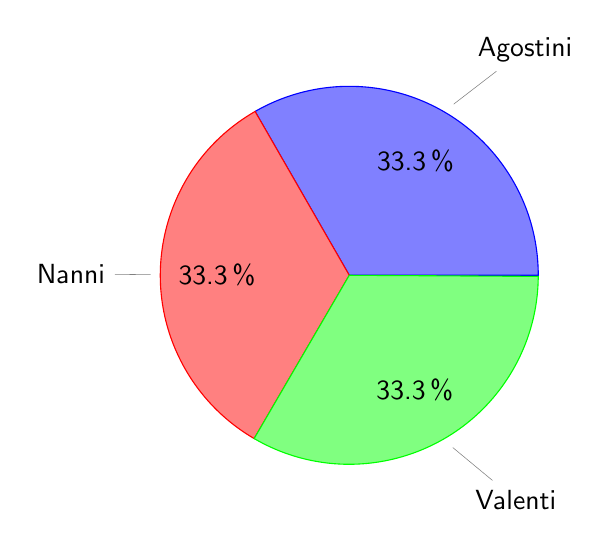
\begin{tikzpicture}[scale=0.8, nodes = {font=\sffamily}]
  \foreach \percent/\name in {
      33.3/Agostini,
      33.3/Nanni,
      33.3/Valenti
    } {
      \ifx\percent\empty\else               % If \percent is empty, do nothing
        \global\advance\cyclecount by 1     % Advance cyclecount
        \global\advance\ind by 1            % Advance list index
        \ifnum3<\cyclecount                 % If cyclecount is larger than list
          \global\cyclecount=0              %   reset cyclecount and
          \global\ind=0                     %   reset list index
        \fi
        \pgfmathparse{\cyclelist[\the\ind]} % Get color from cycle list
        \edef\color{\pgfmathresult}         %   and store as \color
        % Draw angle and set labels
        \draw[fill={\color!50},draw={\color}] (0,0) -- (\angle:\radius)
          arc (\angle:\angle+\percent*3.6:\radius) -- cycle;
        \node at (\angle+0.5*\percent*3.6:0.7*\radius) {\percent\,\%};
        \node[pin=\angle+0.5*\percent*3.6:\name]
          at (\angle+0.5*\percent*3.6:\radius) {};
        \pgfmathparse{\angle+\percent*3.6}  % Advance angle
        \xdef\angle{\pgfmathresult}         %   and store in \angle
      \fi
    };
\end{tikzpicture}
\end{figure}

\newpage
La sua sede legale e sociale è stata stabilita in Albania, presso la città di Tirana all'interno di un ufficio di $ 137 \: m^2 $ \cite{Ufficio}, perchè in questo modo si riescono a sfruttare le opportunità che offre questo paese per attrarre gli investimenti esteri, in particolare:
\begin{itemize}
\item una burocrazia snella ed un sistema fiscale che agevole tramite apposite normative le iniziative imprenditoriali (per dettagli vedere paragrafo~\ref{sec:normative_fiscali_albania});
\item un \textbf{cambio favorevole}. La moneta locale, il \textit{lek} (\textbf{ALL}), presenta il seguente tasso di cambio:
	\begin{center}
		1 \euro : 136,51 ALL\footnote{dati aggiornati al 15/12/2016 (fonte http://it.coinmill.com/ALL\_EUR.html)}
	\end{center}
	
	\begin{tcolorbox}[colframe=blue!75!black,adjusted title=\textbf{Osservazione!}]
		Per nostra semplicità abbiamo eseguito i nostri calcoli in \textit{euro} considerando dati espressi in LEK rappresentativi del tenore di vita a Tirana.
	\end{tcolorbox}

\item una \textbf{posizione geografica strategica} tra i paesi dell'\ac{UE} (Italia e Grecia) e quelli della penisola balcanica (confina con il Montenegro a nord-ovest, il Kosovo a nord-est, la Macedonia ad est ) che permette facilmente di poter espandere la propria presenza nei mercati di questi paesi, senza dimenticare altri potenziali paesi come la Croazia, la Romania o la Bulgaria.
\item la presenza di \textbf{accordi bilaterali} con l'Italia (che costituisce il principale partner commerciale) e con l'\ac{UE} in generale, che favoriscono gli scambi commerciali e, nel nostro caso, permettono di evitare la \textbf{doppia imposizione}\cite{accordialbaniaitalia}. In pratica, gli utili che realizzeremo in Albania andranno a costituire una base imponibile per il pagamento delle tasse soltanto in questo paese e non in Italia.  
\item un altro fattore determinante per la scelta dell'Albania è la forte concentrazione di una comunità italiana all'interno della città di Tirana, permettendo di reperire facilmente un numero di dipendenti con una buona conoscenza della lingua italiana.
\end{itemize}  
\section[Organigramma Aziendale]{Organigramma Aziendale}
La struttura della\textbf{ \ac{ANV S.r.l.}} prevede una struttura gerarchica piramidale, in particolare:
\begin{itemize}

 	\item i \textbf{soci fondatori} ricevono gli utili generati dalla società ripartiti in base alle quote possedute della stessa, adeguano il patrimonio societario in base alle strategie descritte nel piano di investimento annuale presentato dal \textbf{\ac{CEO}} e giudicano l'operato di quest'ultimo sui risultati ottenuti; 
 	
	\item un \textbf{\ac{CEO}} responsabile degli investimenti, a capo del consiglio di amministrazione che prevede oltre ai soci fondatori anche altri 3 manager;
	
	\item \textbf{3 manager} responsabili, ognuno, del funzionamento di una squadra di 10 centralinisti;
	
	\item \textbf{30 centralinisti} suddivisi in due turni da 6 ore lorde (comprensive di 2 pause caffè da 15 minuti ciascuna) in una giornata. 

\end{itemize}  

Tale struttura può essere schematizzata dalla seguente figura:
\newline


\begin{tikzpicture}[
  level 1/.style={sibling distance=55mm},
  edge from parent/.style={->,draw},
  >=latex]

% root of the the initial tree, level 1
\node[root] {CEO}
% The first level, as children of the initial tree
  child {node[level 2] (c1) {Manager \#1}}
  child {node[level 2] (c2) {Manager \#2}}
  child {node[level 2] (c3) {Manager \#3}};

% The second level, relatively positioned nodes
\begin{scope}[every node/.style={level 3}]
\node [below of = c1, xshift=30pt] (c11) {Centralinista \#1};
\node [below of = c11] (c12) {Centralinista ...};
\node [below of = c12] (c13) {Centralinista \#5};

\node [below of = c2, xshift=30pt] (c21) {Centralinista \#6};
\node [below of = c21] (c22) {Centralinista ...};
\node [below of = c22] (c23) {Centralinista \#10};

\node [below of = c3, xshift=30pt] (c31) {Centralinista \#11};
\node [below of = c31] (c32) {Centralinista ...};
\node [below of = c32] (c33) {Centralinista \#15};
\end{scope}

% lines from each level 1 node to every one of its "children"
\foreach \value in {1,2,3}
  \draw[->] (c1.195) |- (c1\value.west);

\foreach \value in {1,...,3}
  \draw[->] (c2.195) |- (c2\value.west);

\foreach \value in {1,...,3}
  \draw[->] (c3.195) |- (c3\value.west);
\end{tikzpicture}

Si può osservare come si tratta di una società di piccole dimensioni adeguata sia alle disponibilità economiche di ciascun socio sia al potenziale ufficio disponibile a Tirana, in quanto già provvisto della maggiorparte delle strutture necessarie al funzionamento di un call center.

\section[Sistelia Group S.r.l.]{Sistelia Group S.r.l.}

Il \textit{Gruppo Sistelia} rappresenta una delle principali realtà tecnologiche italiane, in grado di sviluppare soluzioni di alta tecnologia impiantistica e ingegneristica dei sistemi.
Si occupa della realizzazione di impianti complessi di telecomunicazioni, sistemi integrati \textit{voip}, piattaforme di call center, soluzioni professionali di \textit{webmarketing} e \textit{marketing aziendale}, piattaforma web complesse, soluzioni \textit{e-commerce}, impianti  avanzati di rete, soluzioni software su misura, formazione professionale, \textit{web integrated application}.
Il Gruppo Sistelia è proprietario di marchi prestigiosi che rappresentano un punto di riferimento nei rispettivi settori:
\begin{itemize}
\item VOIP GENIC
\item  ALTENIA
\item  ALMESIA 
\item  CAPITAL MEDIA
\item  ITAL HOLDING
\item RETETURISMO
\item FORMTECNICA
\end{itemize}

Il \textit{Gruppo Sistelia} è la società leader nel mercato italiano specializzata nella realizzazione di piattaforme di telecomunicazioni ed impianti informatizzati. Nello specifico sono specializzati nella realizzazione di impianti e software per call center con centinaia di progetti realizzati non solo in Italia ma anche sul territorio internazionale.
Per la realizzazione di un call center Sistelia fornisce un gruppo di esperti, che si occupano della realizzazione di un impianto completo composto da server centralino, postazioni e tutto il necessario.
Inoltre forniscono un software in grado di gestire le campagne di telemarketing, visionare attraverso un pannello di controllo gli eventuali operatori ed i tabulati delle chiamate, gestire un agenda aziendale condivisa che permetta una facile gestione del call center.

Fornisce un servizio di assistenza ed un supporto non solo tecnico ma anche organizzativo. Inoltre il \textit{Gruppo Sistelia} consiglia attraverso il proprio gruppo di esperti il tipo di personale da assumere per garantire il minimo rischio d'impresa restando al contempo conformi alle vigenti normative del settore.

Il punto cruciale di tutta l'attività di un call center è quello di disporre di validi mandati di lavoro che assicurano alla struttura la produttività nel tempo.
Considerando il mercato attuale un imprenditore che vuole aprire un call center di successo non può' e non deve affidarsi esclusivamente ai classici mandati di telefonia e di energia che risultano allo stato attuale oltre che in completa saturazione, superati e poco interessanti per il cliente finale. 
A tal proposito il \textit{Gruppo Sistelia} fornisce ai vari imprenditori un pacchetto di clienti ottenuti attraverso le varie partnership stabilite con altre aziende, fornendo un mezzo per ottenere un più probabile guadagno ai vari call center. 

Il \textit{Gruppo Sistelia} garantisce i servizi precedentemente descritti anche all'interno di altri paesi poichè vanta alcune filiali anche all'interno di stati quali:
\begin{itemize}
\item Albania
\item Tunisia
\item Croazia
\item Ucraina
\item Romania
\end{itemize}

\subsection{Soluzione Full Sistelia}
\textit{Sistelia} offre due tipi di soluzione per la realizzazione di un call center, che si differenziano per il tipo di preventivo.
Nel nostro caso si è deciso di utilizzare una soluzione di tipo Full poichè in linea con le scelte progettuali proposte in seguito. Qui di seguito mostriamo la tabella relativi ai servizi offerti dal pacchetto Full (vedi figura \ref{fig:full}).
\begin{figure}[htbp]
\centering
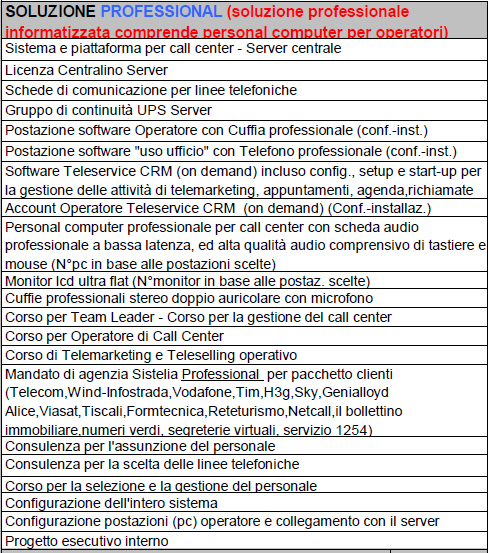
\includegraphics[scale=0.85]{immagini/Full.png}
\caption{Elenco Servizi offerti dalla soluzione Full \label{fig:full}}
\end{figure}
Inoltre mostriamo i costi relativi al numero di postazioni richieste e gli eventuali servizi aggiuntivi (vedi figure \ref{fig:full},\ref{fig:serviziplus}).
Nel nostro caso sono stati scelti i seguenti servizi aggiuntivi:
\begin{itemize}
\item Software per la gestione del personale - configurazione-installazione.
\item Affiancamento e supporto Nostro personale presso Vostra sede.
\item File server per gestione della rete informatica.
\end{itemize}
\begin{figure}[htbp]
\centering
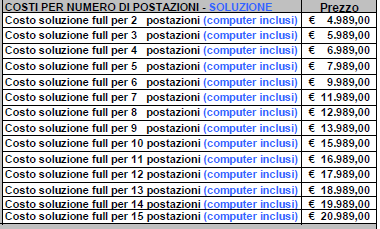
\includegraphics[scale=0.9]{immagini/Postazioni.png}
\caption{Costo della soluzione Full in base al numero di postazioni \label{fig:postazioni}}
\end{figure}
\begin{figure}[htbp]
\centering
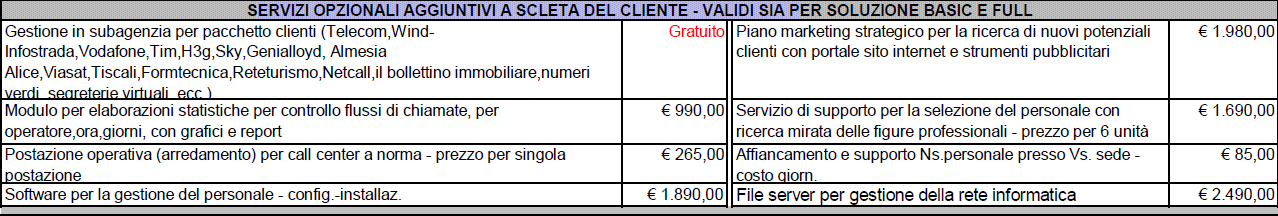
\includegraphics[width=1.15\textwidth,center]{immagini/serviziplus.png}
\caption{Elenco Servizi aggiuntivi  \label{fig:serviziplus}}
\end{figure}


\subsection[ReteTurismo]{ReteTurismo}
ReteTurismo è uno dei partner commerciali del \textit{Gruppo Sistelia} che garantisce una serie di pacchetti di viaggio per tutti gli utenti selezionati. Tale gruppo fornisce un pagamento di \EUR{80} per ogni contratto stipulato.
L'ammontare di crediti contratti verso il \textit{Gruppo Sistelia} verranno riscossi soltanto alla fine del mese corrente.
Tali pacchetti ed i numeri da telefonare sono forniti da \textit{Gruppo Sistelia} verso il call center affiliato garantendo un certo volume di traffico e una più alta probabilità di successo di sottoscrizione.
Per l'analisi dei guadagni generati e del volume di traffico prodotto si rimanda ai paragrafi successivi.